\capitulo{3}{Conceptos teóricos}

Se sintetizarán a continuación algunos de los conceptos teóricos más relevantes para la correcta comprensión del documento.

\section{Apendizaje automático}

Se denomina aprendizaje automático a aquella rama de la inteligencia artificial cuyo objetivo es desarrollar métodos que permitan que un algoritmo mejore su rendimiento mediante la experiencia y procesado de datos. Consecuentemente, los modelos entrenados realizarán predicciones cada vez más precisas como resultado del algoritmo implementado.

Dentro del aprendizaje automático se diferencian tres grandes grupos en función del tipo de entrada que sea consumida: el aprendizaje supervisado (datos etiquetados), el no supervisado (datos no etiquetados) y el semisupervisado (datos etiquetados y no etiquetados), siendo esta última categoría objeto de estudio en este proyecto de investigación. 

\section{Aprendizaje semisupervisado}

Como se ha mencionado anteriormente, se denomina aprendizaje semisupervisado a aquel conjunto de algoritmos que utiliza datos etiquetados y no etiquetados para realizar tareas de aprendizaje. Inicialmente, se pueden diferenciar dos categorías~\cite{engelen2020surveyOnSemiSupervised}: los métodos inductivos, cuyo objetivo principal es construir un clasificador que genere predicciones para cualquier entrada y los métodos transductivos, cuyo poder de predicción está limitado a los objetos utilizados en la fase de entrenamiento.


\begin{figure}[h]
\caption{Clasificación sugerida por~\cite{engelen2020surveyOnSemiSupervised}}
\centering
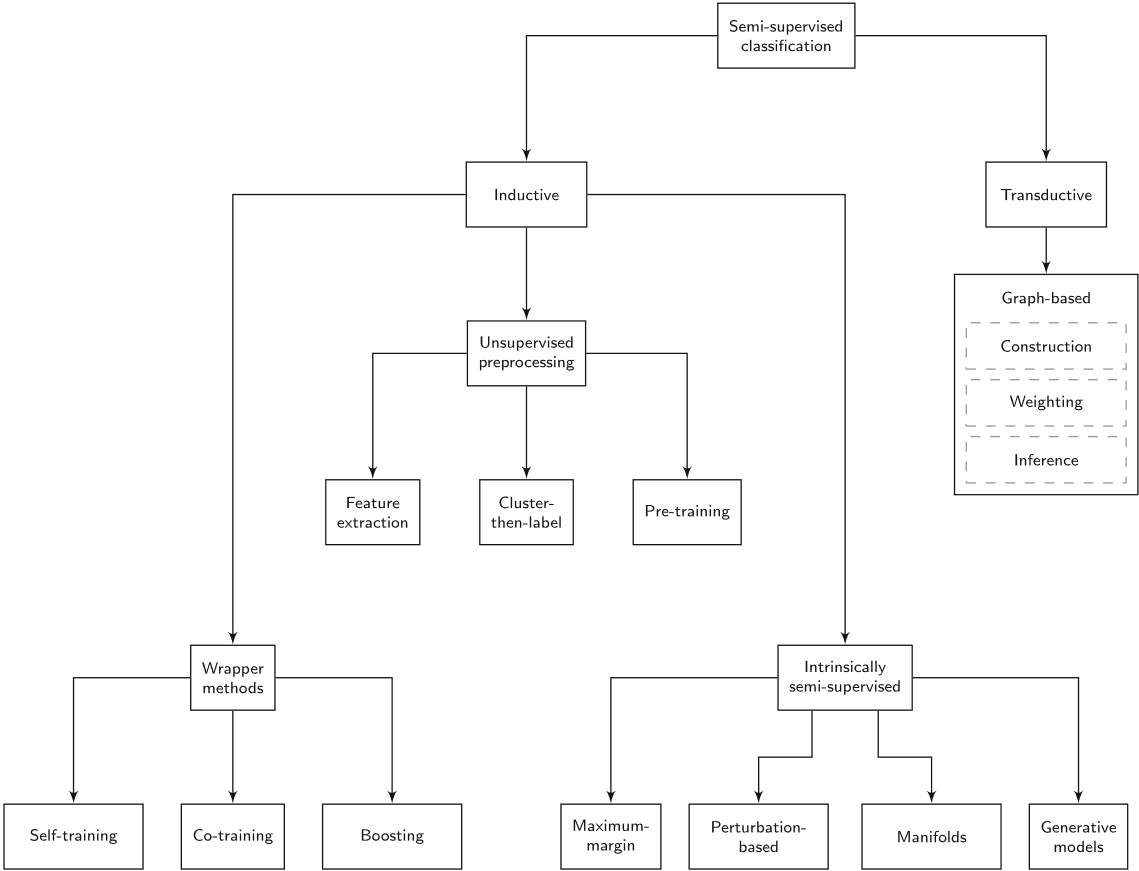
\includegraphics[width=\textwidth]{../img/memoria/esquemaHoos}
\end{figure}

Prescindiendo de los métodos transductivos por ser menos versátiles y útiles en nuestro propósito, los métodos inductivos se subdividen en tres grupos~\cite{engelen2020surveyOnSemiSupervised}: \textit{wrapper methods} (o métodos de envoltura), \textit{unsupervised preprocessing} y \textit{intrinsically semi-supervised}, siendo materia de estudio los métodos de envoltura. 


\subsection{Métodos de envoltura}

Estos modelos utilizan uno o más clasificadores que son entrenados iterativamente con los datos etiquetados de entrada, además de con datos pseudoetiquetados. Se denomina pseudoetiquetado a aquellos datos que inicialmente no estaban etiquetados, pero acabaron estándolo por iteraciones previas de los clasificadores.

Consecuentemente, el procedimiento consta de dos fases que se repiten en cada iteración: el entrenamiento y el pseudoetiquetado. Durante el entrenamiento, los clasificadores se alimentan de datos etiquetados (o pseudoetiquetados). En la fase de pseudoetiquetado, se utilizan datos no etiquetados para que sean procesados por los clasificadores previamente entrenados. 

Dentro de esta categoría, se pueden diferenciar tres grandes grupos: \textit{self-training}, que utilizan únicamente un clasificador, \textit{co-training}~\cite{engelen2020surveyOnSemiSupervised}, que utilizan más de uno y los \textit{pseudo-labelled boosting methods}, que construyen clasificadores individuales que se alimentan de las predicciones más fiables. Se estudiará más en profundidad los métodos \textit{co-training}.

\subsubsection{Co-training y Co-forest}

En estos algoritmos, varios clasificadores son entrenados iterativamente utilizando datos etiquetados y añadiendo las predicciones (resultados) más confiables al conjunto para ser utilizadas en las siguientes iteraciones. Para que los clasificadores sean capaces de generar información distinta, generalmente se divide el conjunto de entrada según alguna característica (no siendo estrictamente necesario).

//TO - DO: Añadir información sobre las dos vistas independientes del co-training (otros métodos no tienen esta limitación)

El llamado \textit{co-forest}, es un modelo dentro de \textit{co-training}. En su desarrollo, se utilizan árboles de decisión (a mayor número mejor resultado), que son entrenados utilizando los datos etiquetados. En cada iteración, además, se añade al conjunto de datos nuevos elementos pseudoetiquetados. Estos elementos son el resultado de los elementos comunes (nuevas etiquetas) del resto de árboles en la fase anterior, y se usan durante una fase de entrenamiento. Sin embargo, se eliminan una vez se ha completado (la siguiente iteración se realiza inicialmente sólo con los datos etiquetados, etc.), consiguiendo así resultados certeros.


\section{\textit{Co-Forest}}

\subsection{Algoritmo}

\subsection{Tratamiento del ruido y teoría de errores}

Como se muestra en~\cite{zhou2021SemisupervisedRecommendationAttack}, de acuerdo con~\cite{noisyExamplesCoforest1988Dana} si el tamaño de los datos utilizados en el entrenamiento (m), la tasa de ruido ($\eta$), el error de la hipótesis en el peor caso ($\epsilon$) y una constante (c) cumplen la relación de la ecuación~\ref{eqn:rel_convergencia_hipotesis}, entonces la hipótesis aprendida por el árbol $h_{i}$ (que minimiza el desacuerdo en un conjunto de muestras de entrenamiento con ruido) converge a la hipótesis verdadera.

\begin{equation}\label{eqn:rel_convergencia_hipotesis} m = \frac{c}{\epsilon^{2}(1-2\eta)^{2}} \end{equation} 

De acuerdo con~\cite{zhou2021SemisupervisedRecommendationAttack}, se puede obtener la función de utilidad mostrada en la ecuación~\ref{eqn:operar_rel_convergencia} operando en la expresión~\ref{eqn:rel_convergencia_hipotesis}.

\begin{equation}\label{eqn:operar_rel_convergencia} f = \frac{c}{\epsilon^{2}} = m(1-2\eta)^{2} \end{equation} 

Como se ha mostrado en el pseudocódigo, en la iteración i-ésima un determinado árbol se entrena con sus datos etiquetados $L_{i}$ y un conjunto de pseudo-etiquetas $L'_{i,t}$. Si se considera que el OOBE cometido en L por $H_{i}$ es $\hat{e}_{i,t}$, entonces se puede estimar que el número de pseudo-etiquetas erróneas en $L'_{i,t}$ equivale a $\hat{e}_{i,t} * W_{i,t}$ (se recuerda al lector que $W_{i,t}$ es el sumatorio de la confianza de predicción (grado de acuerdo) de $H_{i}$ en cada muestra de $L'_{i,t}$). Por lo tanto, la tasa de ruido que se encuentra en $L_{i} \cup L'_{i,t}$ es la estimada por la ecuación~\ref{eqn:ruido_it}, donde $W_0$ y $\eta_0$ son los parámetros correspondientes a L. 

-> CONSULTAR: creo que está bien por ser estimación, pero aún así cada árbol se entrena con un subconjunto aleatorio de L, no con L al completo... Revisar con Alvar.

\begin{equation}\label{eqn:ruido_it} \eta = \frac{\eta_{0}W_{0} + \hat{e}_{i,t}W_{i,t}}{W_{0} + W_{i,t}} \end{equation} 

Concordando con~\ref{eqn:operar_rel_convergencia}, la función de utilidad $f$ es inversamente proporcional a $\epsilon^2$. Por lo tanto, si se quiere reducir el error cometido, se debe aumentar la utilidad de cada árbol en cada iteración~\cite{zhou2021SemisupervisedRecommendationAttack}. Consecuentemente, se debe cumplir la ecuación~\ref{eqn:relacion_e_W}. 

\begin{equation}\label{eqn:relacion_e_W} \frac{\hat{e}_{i,t}}{\widehat{e}_{i, t-1}} < \frac{W_{i,t-1}}{W_{i,t}} < 1 \end{equation} 


\subsubsection{Parámetros del algoritmo}

Intuitivamente se puede deducir la ecuación~\ref{eqn:relacion_e_W}, ya que el error debe disminuir y la confianza de predicción aumentar con cada iteración. Sin embargo, aunque esto se cumpla, puede ser que se deje de cumplir que $\hat{e}_{i,t}W_{i,t} < \hat{e}_{i,t-1}W_{i,t-1}$, ya que puede ocurrir que $ W_{i,t} >>> W_{i,t-1}$. Por este motivo y para cumplir con lo expuesto en~\ref{eqn:relacion_e_W}, se limita $W_{max}$ como se muestra en~\ref{eqn:Wmax} al realizar el muestreo de U en el algoritmo.

\begin{equation}\label{eqn:Wmax} W_{max} = \frac{\hat{e}_{i,t-1}W_{i,t-1}}{\hat{e}_{i, t}} > W_{i,t} \end{equation}


El algoritmo original propuesto por~\cite{originalCoForest2007} y el utilizado en~\cite{zhou2021SemisupervisedRecommendationAttack} dejan, sin embargo, una cuestión pendiente. Como se puede observar en la ecuación~\ref{eqn:Wmax}, $W_{max}$ requiere para calcularse tanto el OOBE como la W obtenida en la iteración anterior, y ambos autores inician W a 0. Esto resulta en que en la primera iteración $W_{max} = 0$ y, por lo tanto, evita que se realice un muestreo de U para pseudo-etiquetar (pararía el algoritmo). En su tésis, Engelen~\cite{engelen2018thesis} propone solucionar este problema iniciando $W = min(\frac{1}{10}|U|, 100)$, aunque destaca que imponer esta constante hace que el impacto de los datos sin etiquetar en el algoritmo dependa profundamente del tamaño del \textit{dataset}.

\section{Ataques a sistemas de recomendación}

Los ataques a los sistemas de recomendación (generalmene denominados \textit{shilling attacks}~\cite{mingdan2018ShillingAttacksAReview} o \textit{profile injection attack}~\cite{Mobasher2006Thesis}) tienen como objetivo manipular las sugerencias que propone un determinado algoritmo para conseguir que un cliente se incline hacia un elemento deseado. Esta alteración del sistema se consigue inyectando perfiles falsos.

Múltiples estudios se han centrado en formalizar las características de estos ataques con el fin de detectarlos. Entre ellas se encuentran~\cite{mingdan2018ShillingAttacksAReview}:

\begin{itemize}
	
	\item \textbf{Intención:} normalmente, se pretende manipular la opinión general acerca de un elemento (ya sea para bien o para mal). Según el objetivo se pueden diferenciar dos tipos de ataques: \textbf{\textit{push attacks}}, que pretenden hacer un objeto más atractivo o \textbf{\textit{nuck attacks}}, cuya intención es la contraria. En caso de que el atacante no busque alterar la opinión acerca de un producto sino restar credibilidad a un sistema (mediante valoraciones aleatorias), se habla de \textbf{\textit{random vandalism}~\cite{Burke2015RobustCollaborative}}.
	
	\item \textbf{Fuerza:} la calidad de los ataques se mide teniendo en cuenta el \textbf{tamaño del relleno} (número de valoraciones asignadas a un perfil atacante, que suele rondar entre el 1 y el 20\% del total de los ítems~\cite{mingdan2018ShillingAttacksAReview}) y el \textbf{tamaño del ataque} (número de perfiles inyectados en el sistema, rondando entre el 1 y el 15\%).
	
	\item \textbf{Coste:} se distinguen dos tipos: \textbf{\textit{knowledge-cost}}, que hace referencia al coste de construir perfiles y \textbf{\textit{deployment-cost}}, que es el número de perfiles que se deben inyectar para conseguir un ataque efectivo~\cite{Mobasher2006Thesis}.
	
\end{itemize}
		
\subsection{Tipos de ataques}

En la actualidad se distinguen multitud de ataques distintos. Con el fin de formalizarlos matemáticamente, se han establecido ciertos conjuntos de interés dependiendo de los ítems que contengan~\cite{zhou2021SemisupervisedRecommendationAttack}.

\begin{itemize}
	
	\item \textbf{$I_S$:} conjunto de ítems seleccionados para recibir un tratamiento especial (puede ser vacío).
	\item \textbf{$I_F$:} conjunto de ítems seleccionados para <<rellenar>>.
	\item \textbf{$I_0$:} conjunto de ítems pertenecientes al sistema de recomendación sin valorar.
	\item \textbf{$I_t$:} conjunto de ítems objetivo.
	
\end{itemize}


\subsubsection{Ataques básicos}

Se distinguen dos tipos: \textit{random attack} y \textit{average attack}~\cite{mingdan2018ShillingAttacksAReview}. Ambos tienen parámetros y características muy similares como se muestra en la tabla \ref{tabla_descripcion_ataques_basicos}. La principal diferencia reside en que el \textit{average attack} es mucho más potente debido a que cuenta con mayor información acerca del sistema: las valoraciones a los ítems de relleno siguen una distribución $\mathcal{N}(\mu_i,\,\sigma_i)$, en lugar de $\mathcal{N}(\mu,\,\sigma)$. Es decir, la valoración para un determinado ítem se adecúa a la distribución concreta de ese ítem en lugar de a la de todo el \textit{dataset}.


\begin{table}\centering
	\resizebox{15cm}{!} {
		\begin{tabular}{c c c c c}\toprule
		Modelo & \textbf{$I_S$:} & Valoración \textbf{$I_F$:} & \textbf{$I_0$:} & Valoración \textbf{$I_t$:} \\ \midrule
	
		Random & $\emptyset$ & \parbox{20em}{Aleatoria siguiendo una distribución normal definida por todas las valoraciones para todos los ítems del sistema $\mathcal{N}(\mu,\,\sigma)$.} & $\emptyset$ & máxima o mínima \\
		
		Average & $\emptyset$ & \parbox{20em}{Aleatoria siguiendo una distribución normal definida por las otras valoraciones para ese ítem en concreto $\mathcal{N}(\mu_i,\,\sigma_i)$.} & $\emptyset$ & máxima o mínima \\
		\bottomrule
		\end{tabular}
	}
	\caption{Descripción de los ataques básicos~\cite{zhou2021SemisupervisedRecommendationAttack}}
	\label{tabla_descripcion_ataques_basicos}	
\end{table}


\subsubsection{Ataques con poco conocimiento del sistema}

Los más populares son \textit{bandwagon attack} (o \textit{popular attack}) y \textit{segment attack}. Sus principales rasgos se ilustran en la tabla \ref{tabla_descripcion_ataques_poco_con}.

La principal característica del \textit{bandwagon attack} es que el conjunto $I_S$ ya no está vacío, sino que contiene algunos de los ítems más populares de la base de datos~\cite{zhou2021SemisupervisedRecommendationAttack}. Estos ítems recibirán también la máxima puntuación posible, de forma que ya no sólo se puntúa el conjunto objetivo. Existe una variante de este ataque llamada \textit{reverse bandwagon attack}, cuyo objetivo es hacer \textit{nuke}. De esta forma, $I_S$ contiene los ítems menos populares y reciben la puntuación mínima (junto con $I_t$).

En el \textit{segment attack}, se realiza un pequeño <<estudio de mercado>> y se introduce en $I_S$ ítems en los que estaría interesado un usuario que fuese a valorar también $I_t$ (de forma que el ataque es más realista).

\begin{table}\centering
		\begin{tabular}{c c c c c}\toprule
			
			Modelo & \textbf{$I_S$:} & Valoración \textbf{$I_F$:} & \textbf{$I_0$:} & Valoración \textbf{$I_t$:} \\ \midrule
			
			\parbox{5em}{Bandwagon (average)} & \parbox{10em} {Ítems populares (valoración máxima) o ítems desfavorecidos (puntuacuón mínima) (reverse)} & \parbox{10em}{Aleatoria siguiendo una distribución normal definida por las otras valoraciones para ese ítem en concreto $\mathcal{N}(\mu_i,\,\sigma_i)$.} & $\emptyset$ & \parbox{5em}{máxima o mínima (reverse)} \\
			
			\parbox{5em}{Bandwagon (random)} & \parbox{10em}{Ítems populares (valoración máxima) o ítems desfavorecidos (puntuacuón mínima) (reverse)} & \parbox{10em}{Aleatoria siguiendo una distribución normal definida por todas las valoraciones para todos los ítems del sistema $\mathcal{N}(\mu,\,\sigma)$.} & $\emptyset$ & \parbox{5em}{máxima o mínima (reverse)} \\
			\bottomrule
		\end{tabular}
	
	\caption{Descripción de los ataques con poco conocimiento del sistema.}
	\label{tabla_descripcion_ataques_poco_con}
\end{table}


\subsubsection{Ataques con gran conocimiento del sistema}

Este tipo de ataques resulta menos relevante que los anteriores debido a la dificultad de su ejecución. En la mayoría de los casos, se necesita una gran cantidad de información, siendo poco realista que se produzca una situación de estas características en la realidad.

Por ejemplo, el llamado \textit{perfect knowledge attack}~\cite{Mobasher2006Thesis} basa su efectividad en reproducir la distribución exacta de la base de datos real (exceptuándo los ítems objetivos). El \textit{sampling attack} construye los perfiles a inyectar basándose en una muestra de perfiles reales~\cite{mingdan2018ShillingAttacksAReview}.

Como se puede intuir, conocer datos estadísticos exactos sobre una base de datos o metadatos asociados a perfiles de usuarios es poco realista (cada vez menos debido a las mayores medidas de seguridad) y por lo tanto estos ataques resultan meramente teóricos.

\subsubsection{Ataques ofuscados}

Los ataques ofuscados~\cite{mingdan2018ShillingAttacksAReview} se basan en intentar <<camuflar>> los perfiles inyectados haciéndolos pasar por reales. Algunas de las características de su implementación se pueden consultar en la tabla \ref{tabla_descripcion_estrategias_ofuscación}

El ataque de \textit{noise injection} introduce a los conjuntos $I_S$ e $I_F$ un <<ruido>> (número aleatorio que sigue una distribución Gaussiana) multiplicado por una constante $\alpha$. \textit{Target shifting} incrementa (o decrementa) en una unidad la valoración de $I_t$ con el fin de crear diferencias entre ataques similares sin influir excesivamente el resultado y el \textit{Average over popular items (AOP)} pretende ofuscar el \textit{average attack} cambiando la forma de selección de $I_F$ (en lugar de seleccionar los ítems del conjunto total de la colección, se seleccionan los $X\%$ ítems más populares).

\begin{table}\centering
	\resizebox{12cm}{!} {
		\begin{tabular}{c c}\toprule
			
			Modelo & Estrategia de ofuscación\\ \midrule
			
			Noise Injection & $\forall i \in I_F \cup I_S: R_i = r_i + aleatorio * \alpha $\\
			Target Shifting & $\forall i \in I_F \cup I_S: R_i = r_i; I_T:$ $r_{max}-1$ o $r_{min}+1$ \\
			AOP & $I_F$ escogido del top ítems más populares.\\
			\bottomrule
		\end{tabular}
	}
	
	\caption{Descripción de las estrategias de ofuscación}
	\label{tabla_descripcion_estrategias_ofuscación}
	
\end{table}

\subsubsection{Otros tipos de ataques}

Además de los ataques previamente ilustrados, existen otros con objetivos más diversos o estrategias distintas. El anteriormente mencionado \textit{random vandalism} (cuya intención únicamente es degradar la calidad del recomendador para causar descontento entre los usuarios) pertenece a esta categoría. Se pueden distinguir, además, ataques basados en copiar comportamientos de usuarios influyentes (modelo \textit{PUA} (\textit{Power User Attack})) o ítems poderosos (modelo \textit{PIA} (\textit{Power Item Attack}))~\cite{mingdan2018ShillingAttacksAReview}. Sin embargo, son menos abundantes.


